\documentclass[12pt]{article}

% --- Standard Packages ---
\usepackage{amsmath, amssymb} 
\usepackage{graphicx} % For including images
\usepackage[margin=1in]{geometry} % For 1-inch margins
\usepackage{setspace} % For 1.5 line spacing
\usepackage{cite} % For bibliography citations
\usepackage[colorlinks=true, linkcolor=blue, citecolor=blue, urlcolor=blue]{hyperref} % Clickable links
\usepackage{appendix} % For appendix formatting
\usepackage[hang,flushmargin]{footmisc} % Optional: Improve footnote formatting
\usepackage{caption} % For caption formatting
\usepackage{titling} % To customize title spacing
\usepackage{titlesec} % To customize section title format

% --- Caption Setup ---
\captionsetup{font=footnotesize} % Set caption font size

% --- Document Information ---
\setlength{\droptitle}{-20pt} % Reduce space above the title
\title{\textbf{Quantum Mechanics of the Cooper Pair Box:\\From Charge Qubit to Transmon}}
\author{Harry Luo}
\date{\small Physics 531 \hspace{2em} May 5, 2025} % Assuming current year for placeholder

% --- Adjust Title Spacing (using the titling package) ---
\pretitle{\begin{center}\large} 
\posttitle{\par\end{center}\vspace{-1.0em}} 
\preauthor{\begin{center}\normalsize}
\postauthor{\par\end{center}\vspace{-1.5em}} 
\predate{\begin{center}\small}
\postdate{\par\end{center}\vspace{-1.5em}}

% --- Spacing ---
\setstretch{1.5} % Set 1.5 line spacing

% --- Reduce font size of sectioning commands ---
% Note: Using \section* will make sections unnumbered. Use \section if numbering is desired.
\titleformat{\section}
    {\large\bfseries} 
    {\thesection}{1em}{}
\titleformat{\subsection}
    {\normalsize\bfseries} 
    {\thesubsection}{1em}{}
\titleformat{\subsubsection}
    {\normalsize\itshape} 
    {\thesubsubsection}{1em}{}

\begin{document}

\maketitle

% --- Introduction ---
\section*{Introduction}

The Cooper Pair Box (CPB) is a foundational superconducting circuit element whose quantum behavior, governed by the \textbf{interplay} between charging energy ($E_C$) and Josephson energy ($E_J$), forms the basis for prevalent qubit designs \cite{Kjaergaard2020}. Its dynamics are described by the Hamiltonian:
\begin{equation}
\hat{H} = 4 E_C (\hat{N} - n_g)^2 - E_J^{(1)} \cos \hat{\phi} - \frac{E_J^{(2)}}{2} \cos (2 \hat{\phi})
\label{eq:main_hamiltonian_final}
\end{equation}
where $\hat{N}$ is the number operator for excess Cooper pairs on a superconducting island, $\hat{\phi}$ is the conjugate phase difference operator ($[\hat{\phi}, \hat{N}] = i$, with $\hbar=1$), and $n_g$ is the tunable gate charge offset. This paper explores the quantum mechanics of this system in the limiting regimes defined by the ratio $E_J/E_C$, connects these regimes to the operation of charge and transmon qubits, and analyzes their key properties based on the solutions derived in Appendix~\ref{app:calculations}.

% --- Limiting Regimes Section ---
\section*{Limiting Regimes and Qubit Properties}

In the charging dominated regime ($E_C \gg E_J^{(1)}, E_J^{(2)}$), the system favors eigenstates $|N\rangle$ with definite Cooper pair numbers (Appendix~\ref{app:part_a}). Near degeneracies, such as at the $n_g=1/2$ charge frustration point, the Josephson coupling $E_J^{(1)}$ mixes the degenerate $|0\rangle$ and $|1\rangle$ states. This creates a two-level system, the \textbf{charge qubit}, whose energy levels exhibit an avoided crossing, as shown in Figure~\ref{fig:avoid_crossing}. A defining characteristic of the charge qubit is its extreme sensitivity to $n_g$, illustrated by the sharp transition in ground state charge probability shown in Figure~\ref{fig:charge_prob}. This sensitivity makes it highly vulnerable to charge noise.

% Figures 1 & 2 side by side using minipage
\begin{figure}[htbp]
    \begin{minipage}[t]{0.48\textwidth}
        \centering
        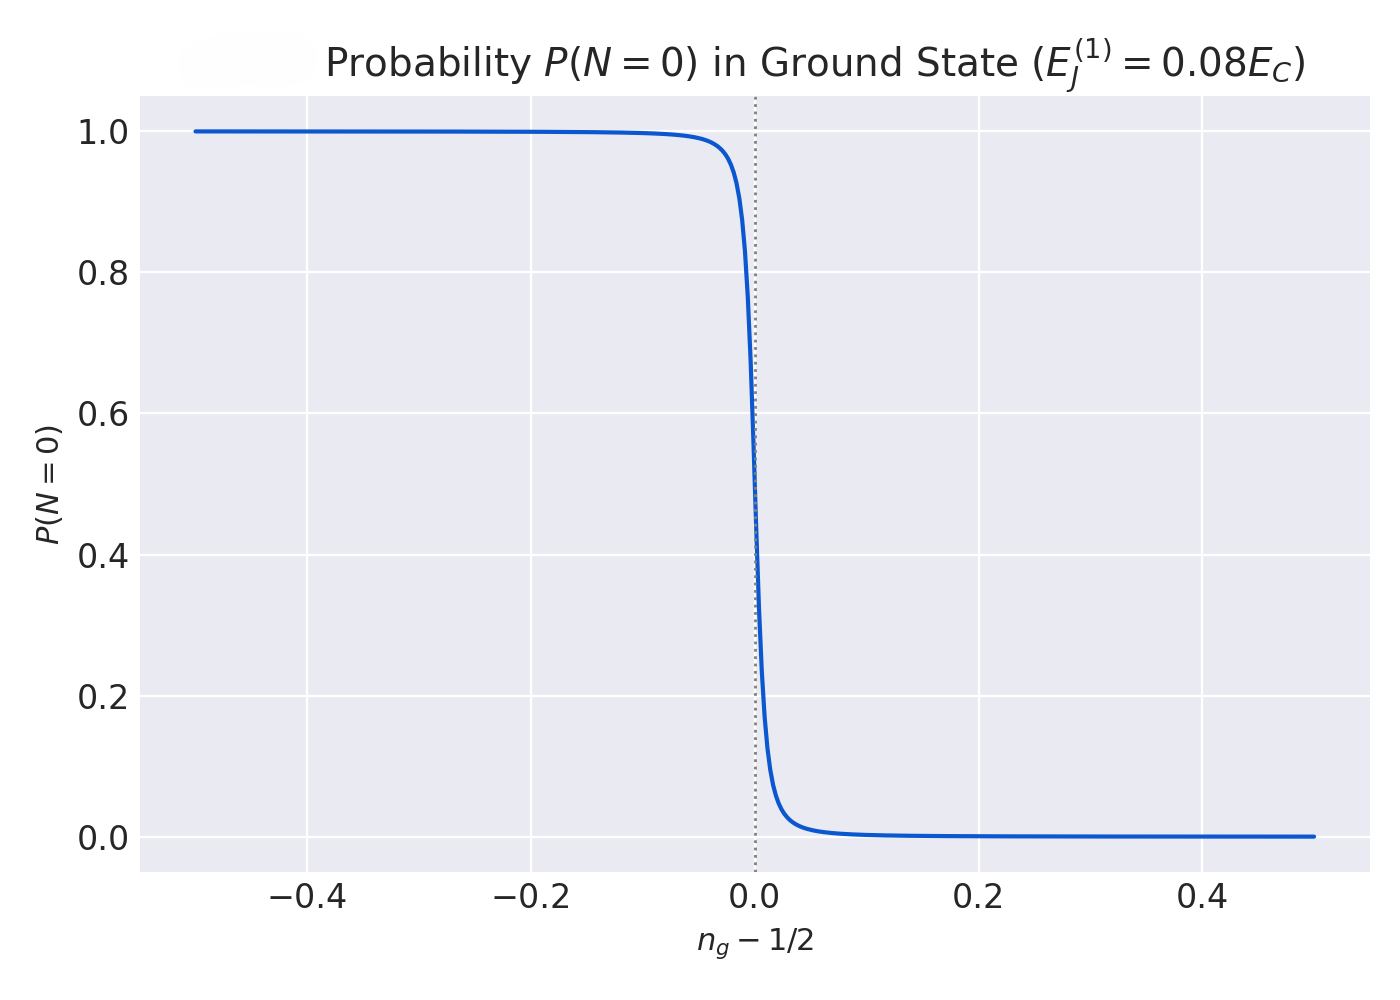
\includegraphics[width=\textwidth]{fig_charge_prob.png}
        \caption{Ground state probability $P(N=0)$ near $n_g=1/2$ for $E_J^{(1)} = 0.08 E_C$, highlighting the charge qubit's sensitivity to $n_g$. Calculation details in Appendix~\ref{app:part_a:subsubsec_iii}.}
        \label{fig:charge_prob}
    \end{minipage}
    \hfill
    \begin{minipage}[t]{0.48\textwidth}
        \centering
        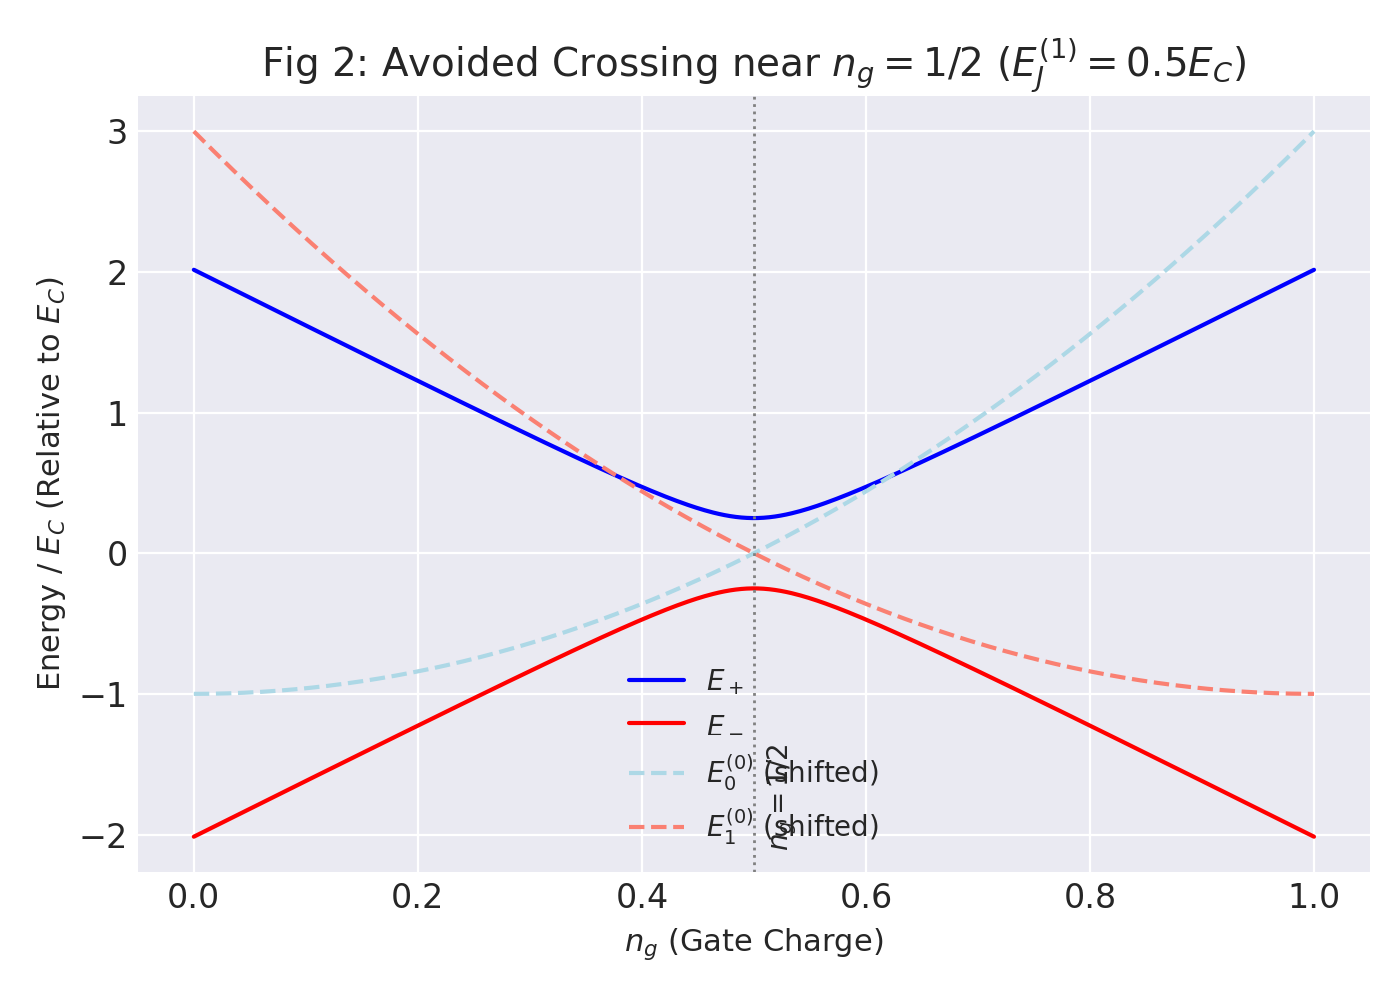
\includegraphics[width=\textwidth]{fig_avoid_crossing.png}
        \caption{Avoided crossing of the lowest two energy levels near the $n_g = 1/2$ degeneracy point, calculated using the effective $2 \times 2$ Hamiltonian for $E_J^{(1)} = 0.5 E_C$. The minimum gap is $E_J^{(1)}$. Derivation in Appendix~\ref{app:part_a:subsubsec_iii}.}
        \label{fig:avoid_crossing}
    \end{minipage}
\end{figure}


In the opposite Josephson dominated regime ($E_J^{(1)}, E_J^{(2)} \gg E_C$, with $n_g=0$), the phase $\phi$ becomes localized near the potential minimum \cite{Koch2007}. The system is well-approximated as an anharmonic oscillator (Appendix~\ref{app:part_b}). Phase localization leads to charge number delocalization, meaning the charge state is highly uncertain. The ground state charge variance $\Delta N^2 = \frac{1}{2X}$ (where $X = \sqrt{8 E_C / (E_J^{(1)} + 2 E_J^{(2)})}$) becomes large, as shown in Figure~\ref{fig:delta_n_variance}. Furthermore, the potential's anharmonicity ensures non-equidistant energy levels ($E_1-E_0 \neq E_2-E_1$), with $\alpha_{anh} \approx -E_C$ (derived in Appendix~\ref{app:part_b:subsubsec_v}), which is vital for qubit addressability.

% Figure 3: Charge Variance (Fixed Label & Caption)
\begin{figure}[htbp]
    \centering
    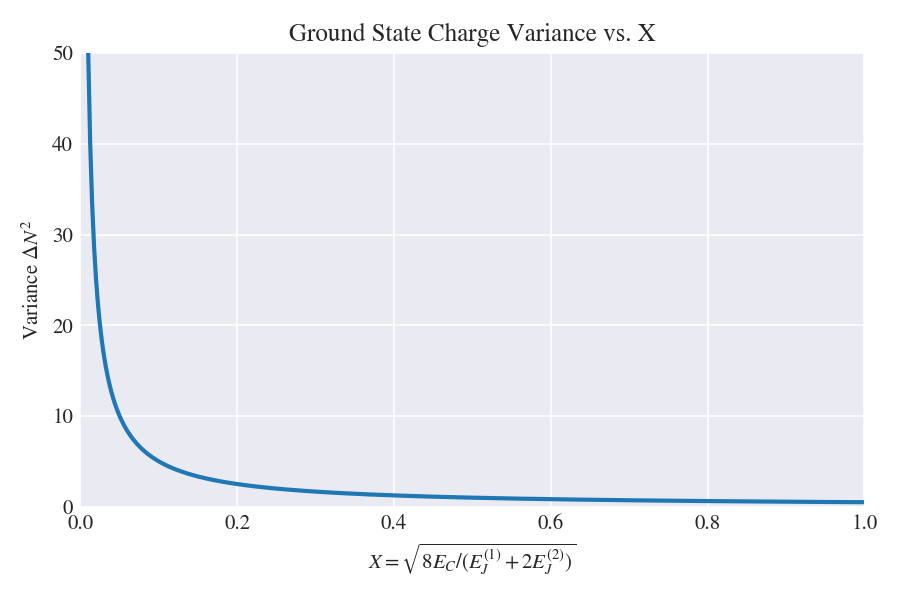
\includegraphics[width=0.65\textwidth]{fig_delta_n_variance.png}
    \caption{Ground state charge variance $\Delta N^2 = 1/(2X)$ vs $X = \sqrt{8 E_C / (E_J^{(1)} + 2 E_J^{(2)})}$. Large $\Delta N^2$ in the transmon limit (small $X$) signifies charge delocalization, key to noise immunity. Calculation in Appendix~\ref{app:part_b:subsubsec_iii}.}
    \label{fig:delta_n_variance} 
\end{figure}

A specific case ($n_g=0, E_J^{(1)}=E_J, E_J^{(2)}=E_J^2/(4E_C)$) admits an exact ground state solution (Appendix~\ref{app:part_c}). Its probability density (Appendix Fig.~\ref{fig:app_exact_prob}) clearly shows the transition from delocalized phase (charge-like, low $E_J/E_C$) to localized phase (transmon-like, high $E_J/E_C$).

% --- Interpretation Section (Revised Text) ---
\section*{Interpretation: Charge vs. Transmon Qubits}

The distinct behaviors in the limiting regimes of the Cooper Pair Box Hamiltonian naturally lead to two types of superconducting qubits \cite{Koch2007, Kjaergaard2020}. In the charging-dominated regime ($E_C \gg E_J$), the \textbf{charge qubit} is formed, typically using the lowest two charge states $|0\rangle$ and $|1\rangle$. Its primary drawback, however, is extreme sensitivity to fluctuations in the gate charge $n_g$. As clearly shown by the sharp transition in the ground state probability (Figure~\ref{fig:charge_prob}) around the $n_g=1/2$ operating point, small variations in $n_g$ significantly alter the qubit's energy splitting (Figure~\ref{fig:avoid_crossing}), making it highly susceptible to environmental charge noise.

Conversely, the \textbf{transmon qubit} operates deep in the Josephson-dominated regime ($E_J \gg E_C$). Its defining characteristic is a significantly suppressed sensitivity to charge noise. This immunity arises because the quantum state becomes delocalized over many charge numbers, leading to a large charge variance ($\Delta N^2 \gg 1$, Figure~\ref{fig:delta_n_variance}). Consequently, the qubit's energy levels become exponentially insensitive to $n_g$, scaling as $\sim e^{-\sqrt{8E_J/E_C}}$ \cite{Koch2007}. This effectively averages out the effect of charge fluctuations, providing crucial protection against decoherence, as schematically illustrated by the flat energy bands in Figure~\ref{fig:transmon_levels}.

While charge insensitivity is paramount, a practical qubit also requires \textbf{anharmonicity}—non-equidistant energy level spacing—to allow selective control of the qubit transition ($0 \leftrightarrow 1$) without exciting higher levels ($1 \leftrightarrow 2$, etc.). The Josephson cosine potential inherently provides this. As calculated from the subleading corrections in the $E_J \gg E_C$ limit (Appendix~\ref{app:part_b:subsubsec_v}), the anharmonicity $\alpha_{anh} = (E_2-E_1) - (E_1-E_0)$ is finite and approximately equal to $-E_C$. This non-zero $\alpha_{anh}$ ensures the distinct transition frequencies necessary for high-fidelity qubit operations.

The design of an effective transmon therefore involves managing the trade-off between maximizing charge insensitivity (favoring large $E_J/E_C$) and maintaining sufficient anharmonicity (which is roughly constant at $-E_C$ in this regime). Figure~\ref{fig:anharm_vs_dispersion} perfectly encapsulates this critical relationship. Panel (a) demonstrates that the anharmonicity $\alpha$ quickly saturates near the required value of $-E_C$ for $E_J/E_C \gtrsim 10$. Panel (b) simultaneously shows the desired exponential decrease in charge dispersion (the sensitivity to $n_g$). Together, these plots illustrate how operating at a sufficiently large ratio (e.g., $E_J/E_C$ in the range 20-100 \cite{Kjaergaard2020}) allows the transmon to achieve substantial noise immunity while preserving the essential anharmonicity for control, fulfilling the design goals implicit in the project requirements (parts b.v and d).

% Figure 4: Anharmonicity vs Dispersion (Old Fig 3)
\begin{figure}[htbp]
    \centering
    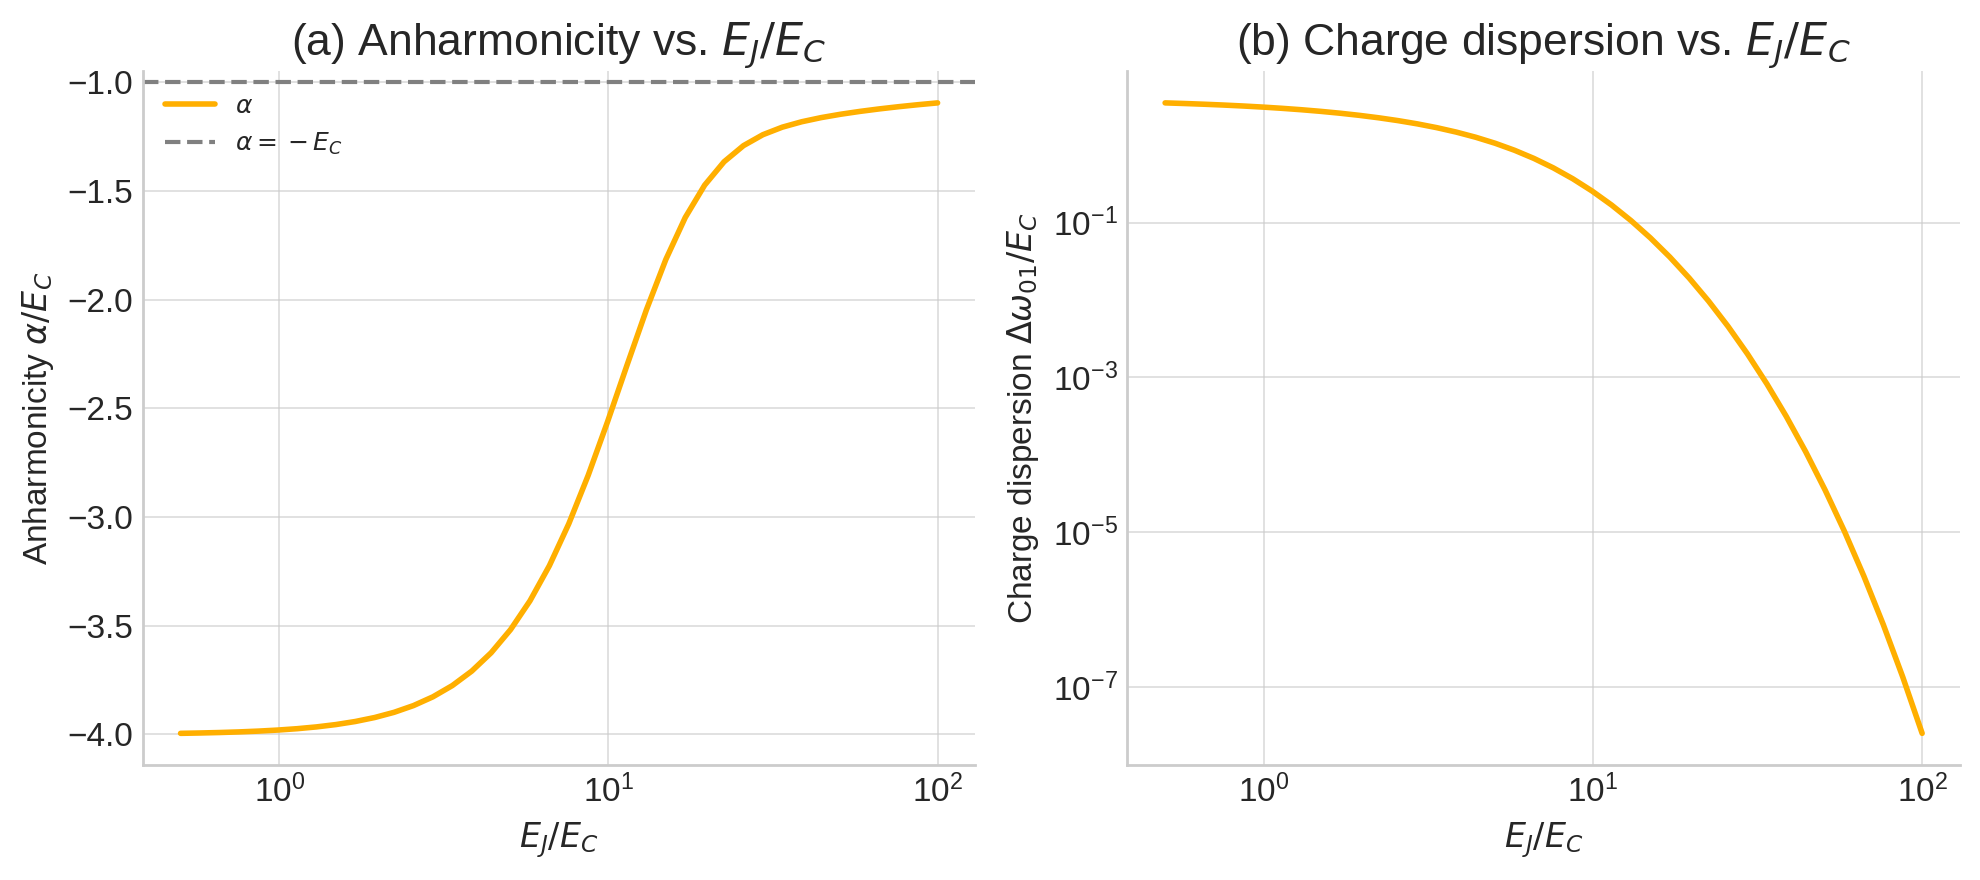
\includegraphics[width=0.95\textwidth]{fig_anharm_dispersion.png}
    \caption{Trade-off between anharmonicity and charge dispersion as a function of the energy ratio $E_J/E_C$. 
    (a) Anharmonicity $\alpha = (E_2-E_1)-(E_1-E_0)$ rapidly approaches the asymptotic value $\alpha \approx -E_C$, sufficient for selective driving. 
    (b) Charge dispersion $\Delta\omega_{01}$ (representing $n_g$ sensitivity) decays exponentially $\propto\exp[-\sqrt{8E_J/E_C}]$ (trend from \cite{Koch2007}), enabling noise immunity.}
    \label{fig:anharm_vs_dispersion} 
\end{figure}

% Figure 5: Transmon Level Sketch (Old Fig 4)
\begin{figure}[htbp] 
    \centering
    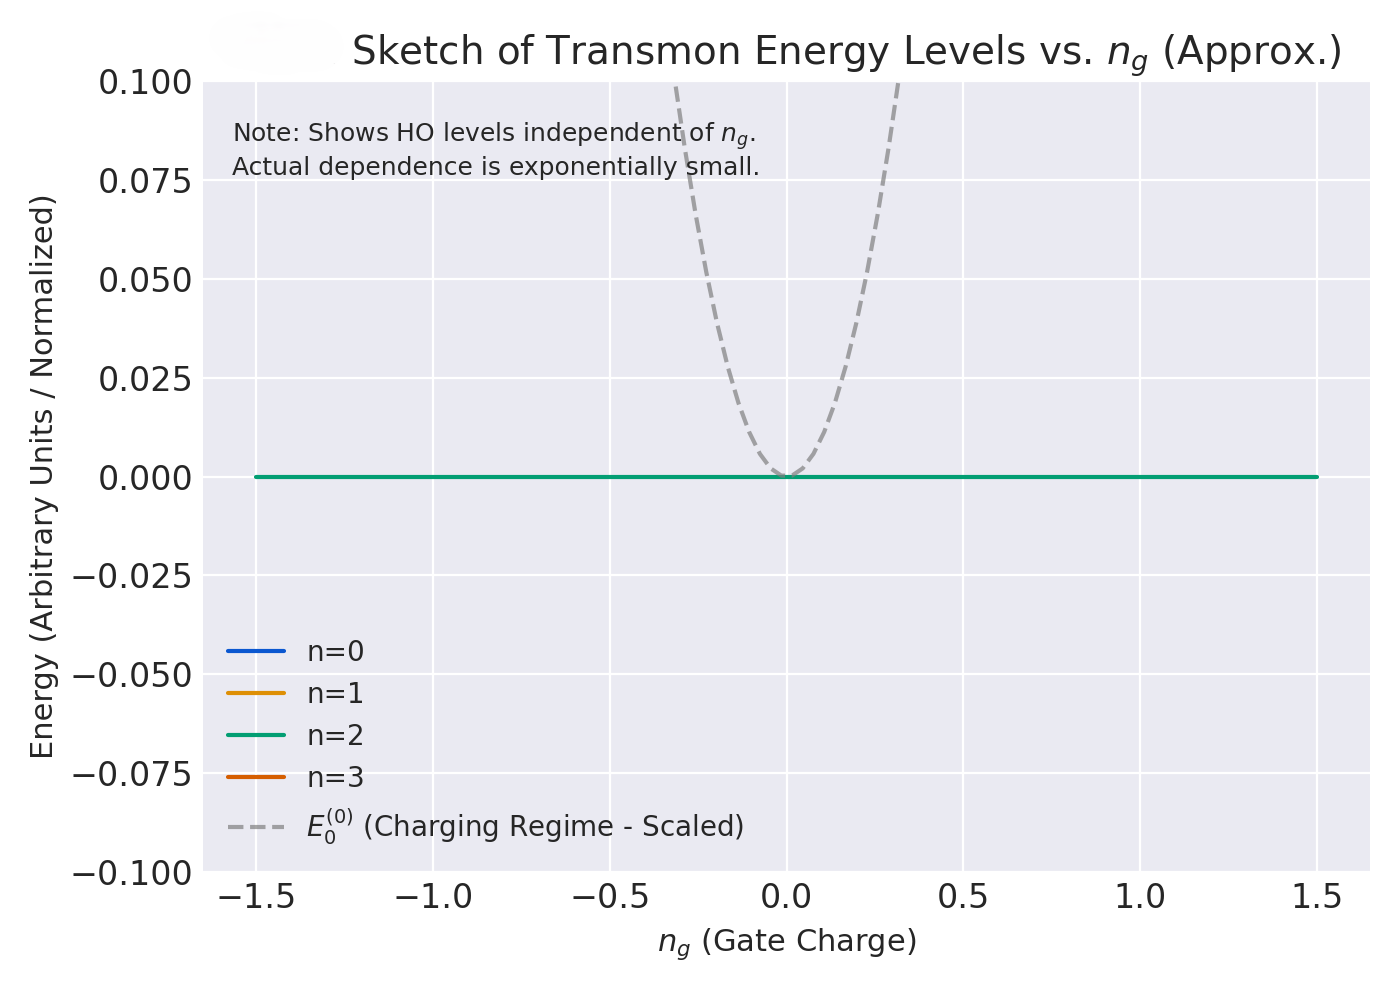
\includegraphics[width=0.65\textwidth]{fig_transmon_levels.png}
    \caption{Sketch comparing the flat (charge-insensitive) energy levels of the transmon ($E_J \gg E_C$) with the parabolic (charge-sensitive) levels of the charge qubit regime.}
    \label{fig:transmon_levels} 
\end{figure}

% --- Conclusion ---
\section*{Conclusion}

The $E_J/E_C$ ratio fundamentally governs the Cooper Pair Box's quantum behavior, dictating the tradeoff between charge sensitivity and phase localization. The charge qubit regime ($E_C \gg E_J$) suffers from charge noise, while the transmon regime ($E_J \gg E_C$) achieves noise resilience through charge delocalization. This resilience, combined with the essential anharmonicity provided by the Josephson potential, makes the transmon a robust and widely implemented superconducting qubit architecture.

% --- Bibliography ---
\begin{thebibliography}{9}
    \bibitem{Koch2007} 
    J. Koch, T. M. Yu, J. Gambetta, A. A. Houck, D. I. Schuster, J. Majer, A. Blais, M. H. Devoret, S. M. Girvin, and R. J. Schoelkopf, 
    "Charge-insensitive qubit design derived from the Cooper pair box," 
    \textit{Physical Review A} \textbf{76}, 042319 (2007).

    \bibitem{Kjaergaard2020} 
    M. Kjaergaard, M. E. Schwartz, J. Braumüller, P. Krantz, J. I.-J. Wang, S. Gustavsson, and W. D. Oliver, 
    "Superconducting Qubits: Current State of Play," 
    \textit{Annual Review of Condensed Matter Physics} \textbf{11}, 369–395 (2020).
\end{thebibliography}

\newpage 
% --- Appendix ---
\begin{appendices}
\section{Detailed Calculations}
\label{app:calculations}

Here we provide the detailed derivations supporting the results presented in the main text, following the structure of the project requirements. We use units where $\hbar=1$.

% --- Appendix Part (a) ---
\subsection[Part (a): Charging Dominated Regime]{Part (a): Charging Dominated Regime ($E_C \gg E_J^{(1)}, E_J^{(2)}$)}
\label{app:part_a}

\subsubsection*{a.i) Eigenstates, Eigenvalues, and Probability Density ($E_J^{(1,2)}=0$)}
\label{app:part_a:subsubsec_i}
The Hamiltonian is $\hat{H}_0 = 4 E_C (\hat{N} - n_g)^2$. Eigenstates are $|N\rangle$ ($\hat{N}|N\rangle = N|N\rangle, N \in \mathbb{Z}$). Eigenvalues:
\begin{equation}
E_N^{(0)}(n_g) = 4 E_C (N - n_g)^2
\label{eq:app_E_N_0_app} 
\end{equation}
These levels are plotted in Figure~\ref{fig:app_charge_levels}. The eigenfunction $\psi_N(\phi) = \frac{1}{\sqrt{2\pi}} e^{i N \phi}$ yields uniform phase probability density $p_N(\phi) = 1/(2\pi)$.

% Appendix Figure 5 (Old Fig 5)
\begin{figure}[htbp]
    \centering
    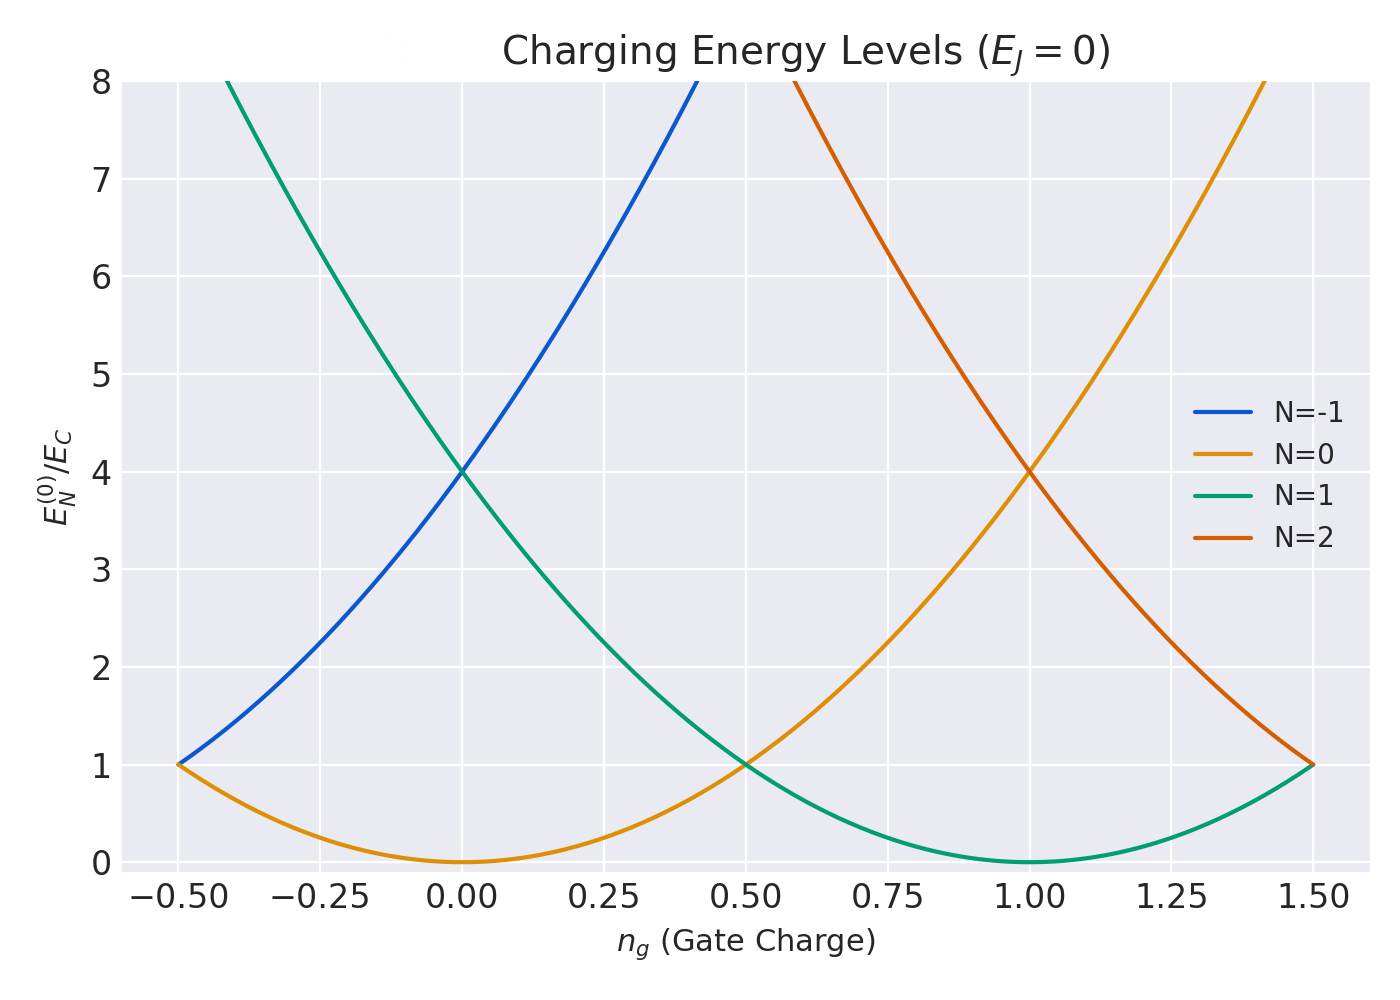
\includegraphics[width=0.6\textwidth]{fig_charge_levels.png}
    \caption{Charging energy levels $E_N^{(0)}/E_C$ versus $n_g$ for $E_J=0$.}
    \label{fig:app_charge_levels}
\end{figure}

\subsubsection*{a.ii) Perturbation Theory Correction at $n_g=0$}
\label{app:part_a:subsubsec_ii}
Perturbation $V = -E_J^{(1)} \cos \hat{\phi} - \frac{E_J^{(2)}}{2} \cos (2 \hat{\phi})$. First-order correction $E_0^{(1)} = 0$. Second-order correction $E_0^{(2)} = \sum_{N \neq 0} \frac{|\langle N | V | 0 \rangle|^2}{E_0^{(0)} - E_N^{(0)}}$. Using matrix elements $\langle \pm 1 | V | 0 \rangle = -E_J^{(1)}/2$ and $\langle \pm 2 | V | 0 \rangle = -E_J^{(2)}/4$:
\begin{equation}
E_0^{(2)} = -\frac{(E_J^{(1)})^2}{8 E_C} - \frac{(E_J^{(2)})^2}{128 E_C}
\end{equation}
This standard perturbation approach breaks down near degeneracies (half-integer $n_g$), where the perturbation's effect is strongest.

\subsubsection*{a.iii) Charge Qubit near $n_g=1/2$}
\label{app:part_a:subsubsec_iii}
In the subspace $\{|0\rangle, |1\rangle\}$ near $n_g=1/2$, the effective Hamiltonian (subtracting $E_C I$) is $H_{\text{eff}} \approx \epsilon_0 \hat{\sigma}_z - \frac{E_J^{(1)}}{2} \hat{\sigma}_x$, where $\epsilon_0 = 4 E_C (n_g - 1/2)$. Eigenvalues $E_{\pm} = \pm \sqrt{\epsilon_0^2 + (E_J^{(1)}/2)^2}$, show an avoided crossing (plotted in Figure~\ref{fig:avoid_crossing} in the main text). 
Ground state ($E_-$) probability in state $|0\rangle$:
\begin{equation}
P(N=0) = \frac{1}{2} \left( 1 - \frac{\epsilon_0}{\sqrt{\epsilon_0^2 + (E_J^{(1)}/2)^2}} \right) 
\end{equation}
This is plotted in Figure~\ref{fig:charge_prob} in the main text.

% --- Appendix Part (b) ---
\subsection[Part (b): Josephson Dominated Regime]{Part (b): Josephson Dominated Regime ($E_J^{(1)}, E_J^{(2)} \gg E_C$, $n_g=0$)}
\label{app:part_b}

\subsubsection*{b.i) Harmonic Oscillator Approximation: Levels and Wavefunctions}
\label{app:part_b:subsubsec_i}
Expanding $V(\phi) = -E_J^{(1)} \cos \phi - \frac{E_J^{(2)}}{2} \cos (2 \phi)$ around $\phi=0$ yields $V(\phi) \approx V(0) + \frac{1}{2} k \phi^2$, with $V(0) = -E_J^{(1)} - E_J^{(2)}/2$ and $k = E_J^{(1)} + 2 E_J^{(2)}$. $\hat{H} \approx V(0) + 4 E_C \hat{N}^2 + \frac{1}{2} k \hat{\phi}^2$ describes a HO with mass $m^* = 1/(8E_C)$ and frequency $\omega = \sqrt{8 E_C k}$. Levels: $E_n^{(HO)} = V(0) + \omega(n+1/2)$. Wavefunctions $\psi_n^{(HO)}(\phi)$ involve Hermite polynomials $H_n$ and width $\alpha = \left( \frac{k}{8 E_C} \right)^{1/4}$. First three explicit forms:
\begin{align*}
\psi_0^{(HO)}(\phi) &= (\alpha^2/\pi)^{1/4} e^{-\alpha^2\phi^2/2} \\
\psi_1^{(HO)}(\phi) &= (\alpha^2/\pi)^{1/4} \sqrt{2}\alpha\phi e^{-\alpha^2\phi^2/2} \\
\psi_2^{(HO)}(\phi) &= (\alpha^2/\pi)^{1/4} \frac{1}{\sqrt{2}} (2(\alpha\phi)^2 - 1) e^{-\alpha^2\phi^2/2} 
\end{align*}

\subsubsection*{b.ii) Probability Density Plot}
\label{app:part_b:subsubsec_ii}
The probability densities $p_n(\phi)=|\psi_n^{(HO)}(\phi)|^2$ for $n=0,1,2$ are plotted in Figure~\ref{fig:app_ho_probs}, using $\alpha^2=10$ as required for $E_C = (E_J^{(1)}+2E_J^{(2)})/800$.

% Appendix Figure 6 (Old Fig 8)
\begin{figure}[htbp]
    \centering
    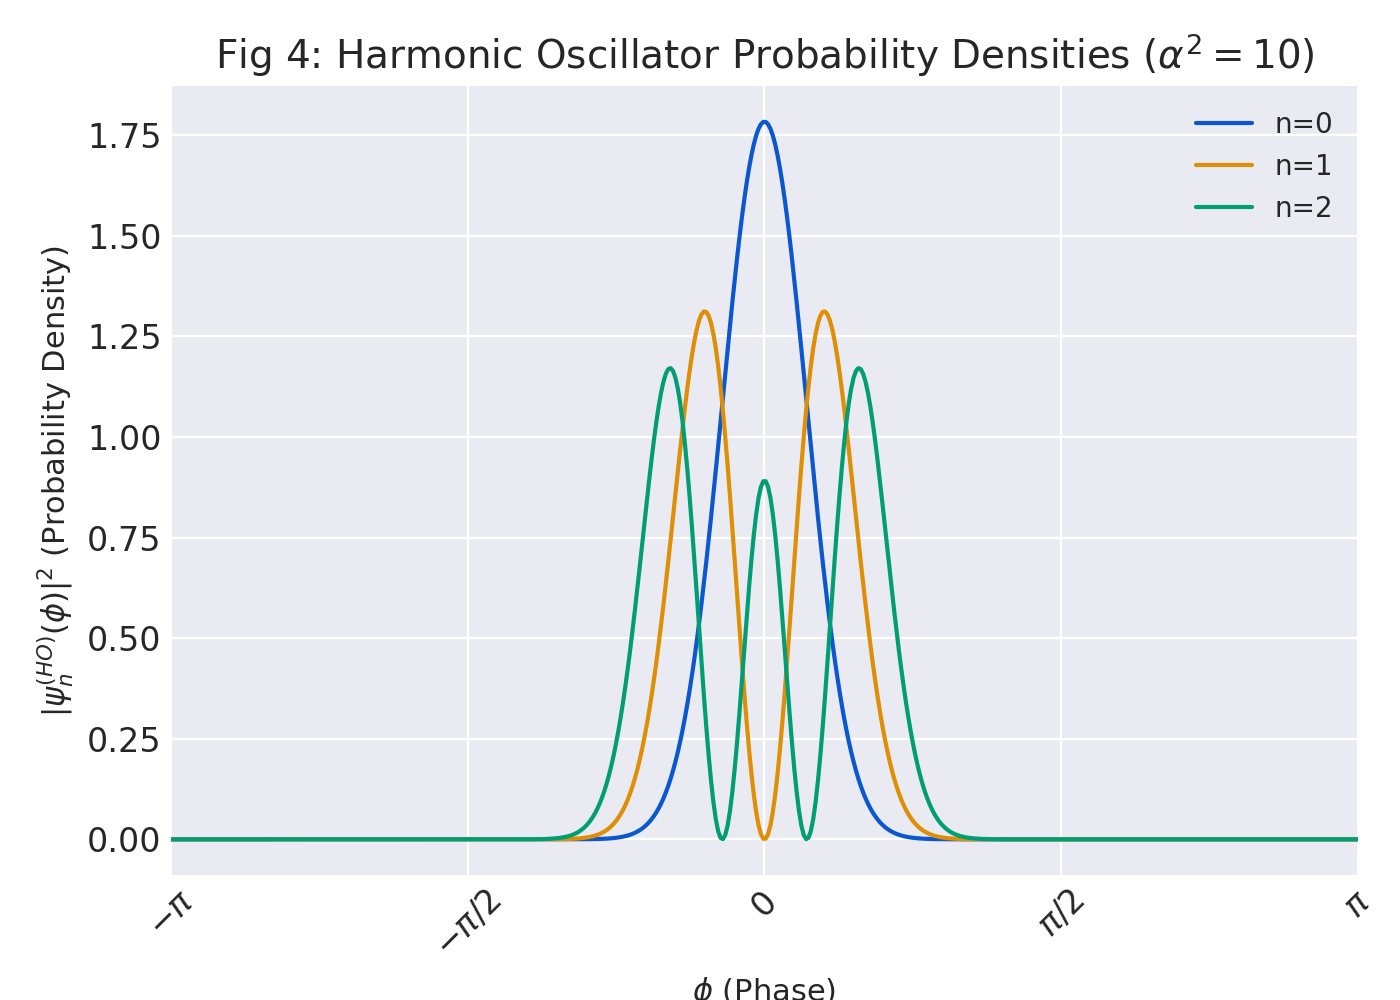
\includegraphics[width=0.6\textwidth]{fig_ho_prob.png} 
    \caption{Approximate HO probability densities $p_n(\phi)$ for $n=0,1,2$ with $\alpha^2=10$.}
    \label{fig:app_ho_probs} 
\end{figure}

\subsubsection*{b.iii) Charge Expectation Value and Variance}
\label{app:part_b:subsubsec_iii}
Ground state average $\langle \hat{N} \rangle_0 = 0$. Variance $\Delta N^2 = \langle \hat{N}^2 \rangle_0$. From $\langle KE \rangle_0 = 4 E_C \langle \hat{N}^2 \rangle_0$ and $\langle KE \rangle_0 = \omega/4$ (HO ground state): $\langle \hat{N}^2 \rangle_0 = \frac{\omega}{16 E_C}$. Standard deviation $\Delta N = \sqrt{\frac{\omega}{16 E_C}}$. With $X = \sqrt{8 E_C / k}$:
\begin{equation}
\Delta N = \sqrt{\frac{1}{2X}}, \quad \Delta N^2 = \frac{1}{2X}
\end{equation}
The variance $\Delta N^2$ is plotted in Figure~\ref{fig:delta_n_variance} in the main text. 
% Removed duplicate plot from appendix

\subsubsection*{b.iv) Subleading Correction to Energy Levels}
\label{app:part_b:subsubsec_iv}
Perturbation $V_{pert} = -\frac{E_J^{(1)} + 8 E_J^{(2)}}{24} \hat{\phi}^4$. First-order correction $E_n^{(1)} = \langle n | V_{pert} | n \rangle$. Using $\langle n | \hat{\phi}^4 | n \rangle = (\frac{4E_C}{\omega})^2 (6n^2 + 6n + 3)$:
\begin{equation}
E_n^{(1)} = - C (6n^2 + 6n + 3), \quad \text{where} \quad C = \frac{E_C (E_J^{(1)} + 8 E_J^{(2)})}{12 (E_J^{(1)} + 2 E_J^{(2)})}
\label{eq:app_energy_corr_app} 
\end{equation}
Corrections for first three levels: $E_0^{(1)} = -3C$, $E_1^{(1)} = -15C$, $E_2^{(1)} = -39C$.

\subsubsection*{b.v) Interpretation: Are Levels Equidistant?}
\label{app:part_b:subsubsec_v}
The anharmonicity is $\alpha_{anh} = (E_2 - E_1) - (E_1 - E_0) \approx E_2^{(1)} - 2E_1^{(1)} + E_0^{(1)} = (-39C) - 2(-15C) + (-3C) = -12C$.
\begin{equation}
\alpha_{anh} = - E_C \frac{E_J^{(1)} + 8 E_J^{(2)}}{E_J^{(1)} + 2 E_J^{(2)}}
\end{equation}
Since $\alpha_{anh} \neq 0$, the energy levels are not equidistant. The spacing decreases with $n$ ($\alpha_{anh} < 0$). This allows selective driving of the $0 \leftrightarrow 1$ qubit transition.

% --- Appendix Part (c) ---
\subsection[Part (c): Exactly Solvable Case]{Part (c): Exactly Solvable Case ($E_J^{(1)}=E_J, E_J^{(2)}=E_J^2/(4E_C)$)}
\label{app:part_c}

With $n_g = 0$ and the specified $E_J^{(1,2)}$, the exact ground state energy is $E_0 = -E_J^2 / (8 E_C)$. The normalized probability density is:
\begin{equation}
p(\phi) = \frac{\exp(\frac{E_J}{2 E_C} \cos \phi)}{2 \pi I_0(E_J / (2 E_C))}
\end{equation}
where $I_0$ is the modified Bessel function. This is plotted in Figure~\ref{fig:app_exact_prob} for the required $E_J/E_C$ values.
Comparison: This $E_0$ matches $E_0^{(2)}$ from Appendix~\ref{app:part_a:subsubsec_ii} if $E_J^{(2)}=0$. It differs from the HO approximation $E_0^{(HO)} \approx -(E_J + \frac{E_J^2}{8 E_C}) + \sqrt{2 E_C E_J + E_J^2}$.

% Appendix Figure 7 (Old Fig 9)
\begin{figure}[htbp]
    \centering
    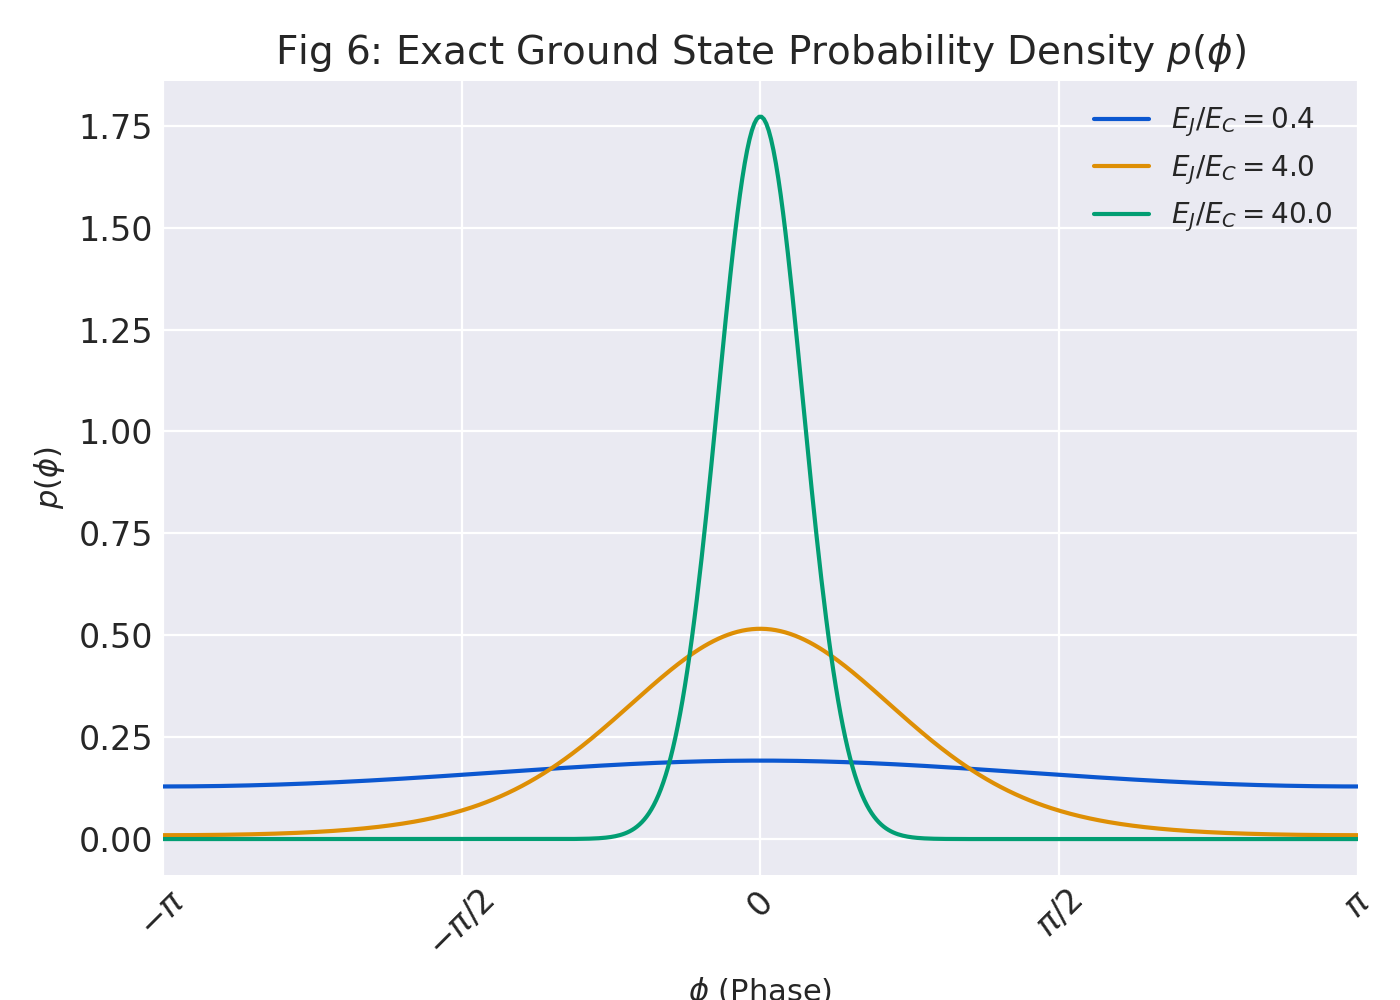
\includegraphics[width=0.6\textwidth]{fig_exact_prob.png}
    \caption{Exact ground state probability density $p(\phi)$ for $E_J/E_C = 0.4, 4.0, 40.0$.}
    \label{fig:app_exact_prob}
\end{figure}

\end{appendices}

\end{document}